\section[Algoritmo Bruto]{Algoritmo Bruto}
\begin{frame}[plain]
	\frametitle{Resolución}
		\begin{exampleblock}{Estrategia de resolución}
			Recorremos la estructura de datos desde el inicio y buscamos el \textbf{primer y único} elemento máximo que encontremos.
		\end{exampleblock}
		
\end{frame}		




\begin{frame}[plain]
	\frametitle{Breve explicación}
		\begin{figure}[htb]
		\begin{center}
		\begin{picture}(160,0)
		\put(-86,-70){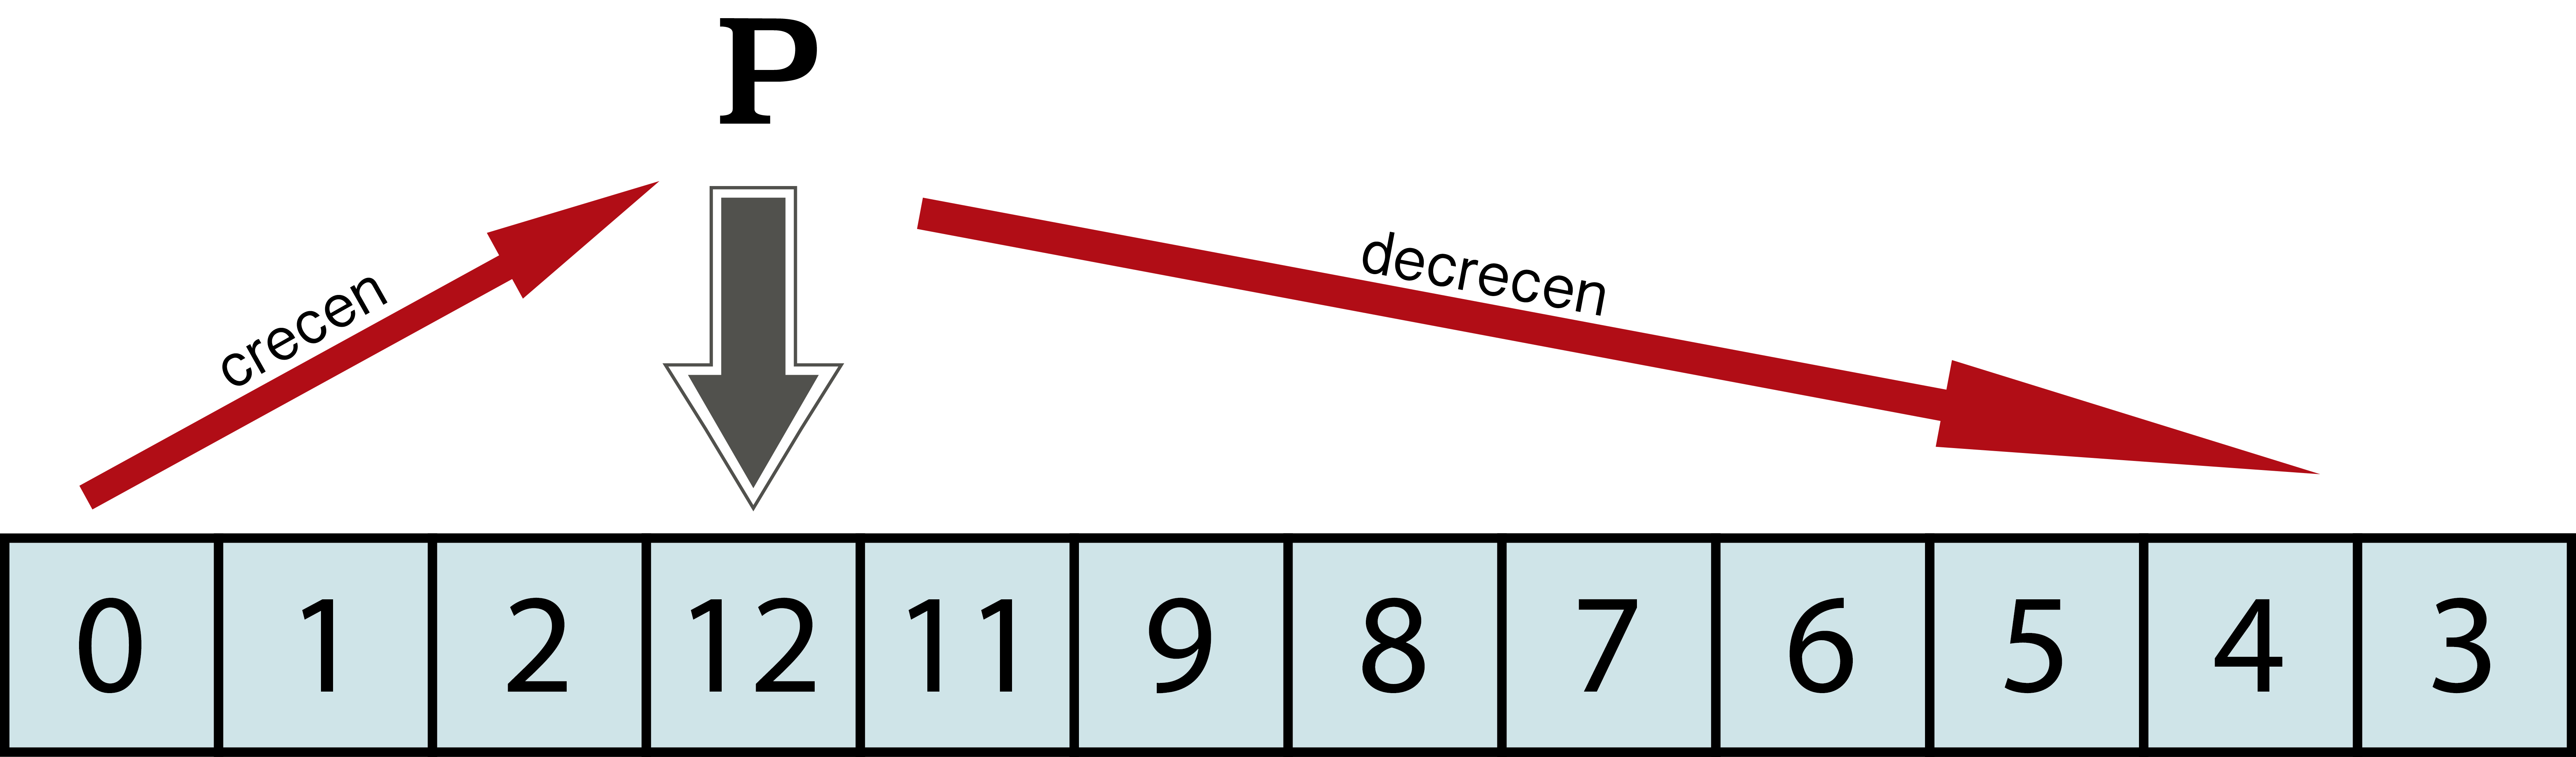
\includegraphics[width=11.5cm,height=4.0cm]{Images/Explicacion}}
		\end{picture}
		\end{center}
		\end{figure}
		
\end{frame}	




\begin{frame}[fragile]
	\frametitle{Algoritmo Bruto - Implementación}
	\lstset{language=C++,
                basicstyle=\ttfamily,
                tabsize=3, 
				showstringspaces=false,
				extendedchars=true,
                keywordstyle=\color{blue}\ttfamily,
                stringstyle=\color{red}\ttfamily,
                commentstyle=\color{yellow}\ttfamily,
                morecomment=[l][\color{magenta}]{\#}
     }
			\vspace*{-0.1in}
\begin{lstlisting}
int unimodalBruto(vector<int> v, int size){
bool found = false;
int pos = 0;

for(int i=0; i< size-1 && !found; i++)
   if(v[i]>v[i+1]){
      pos = i;
      found = true;
   }
    
if(found == false)
	pos = size-1;
return pos;
}

			\end{lstlisting}
	
	
			
\end{frame}	


\begin{frame}[plain]
	\frametitle{Breve explicación}
		\begin{figure}[htb]
		\begin{center}
		\begin{picture}(160,0)
		\put(-50,-110){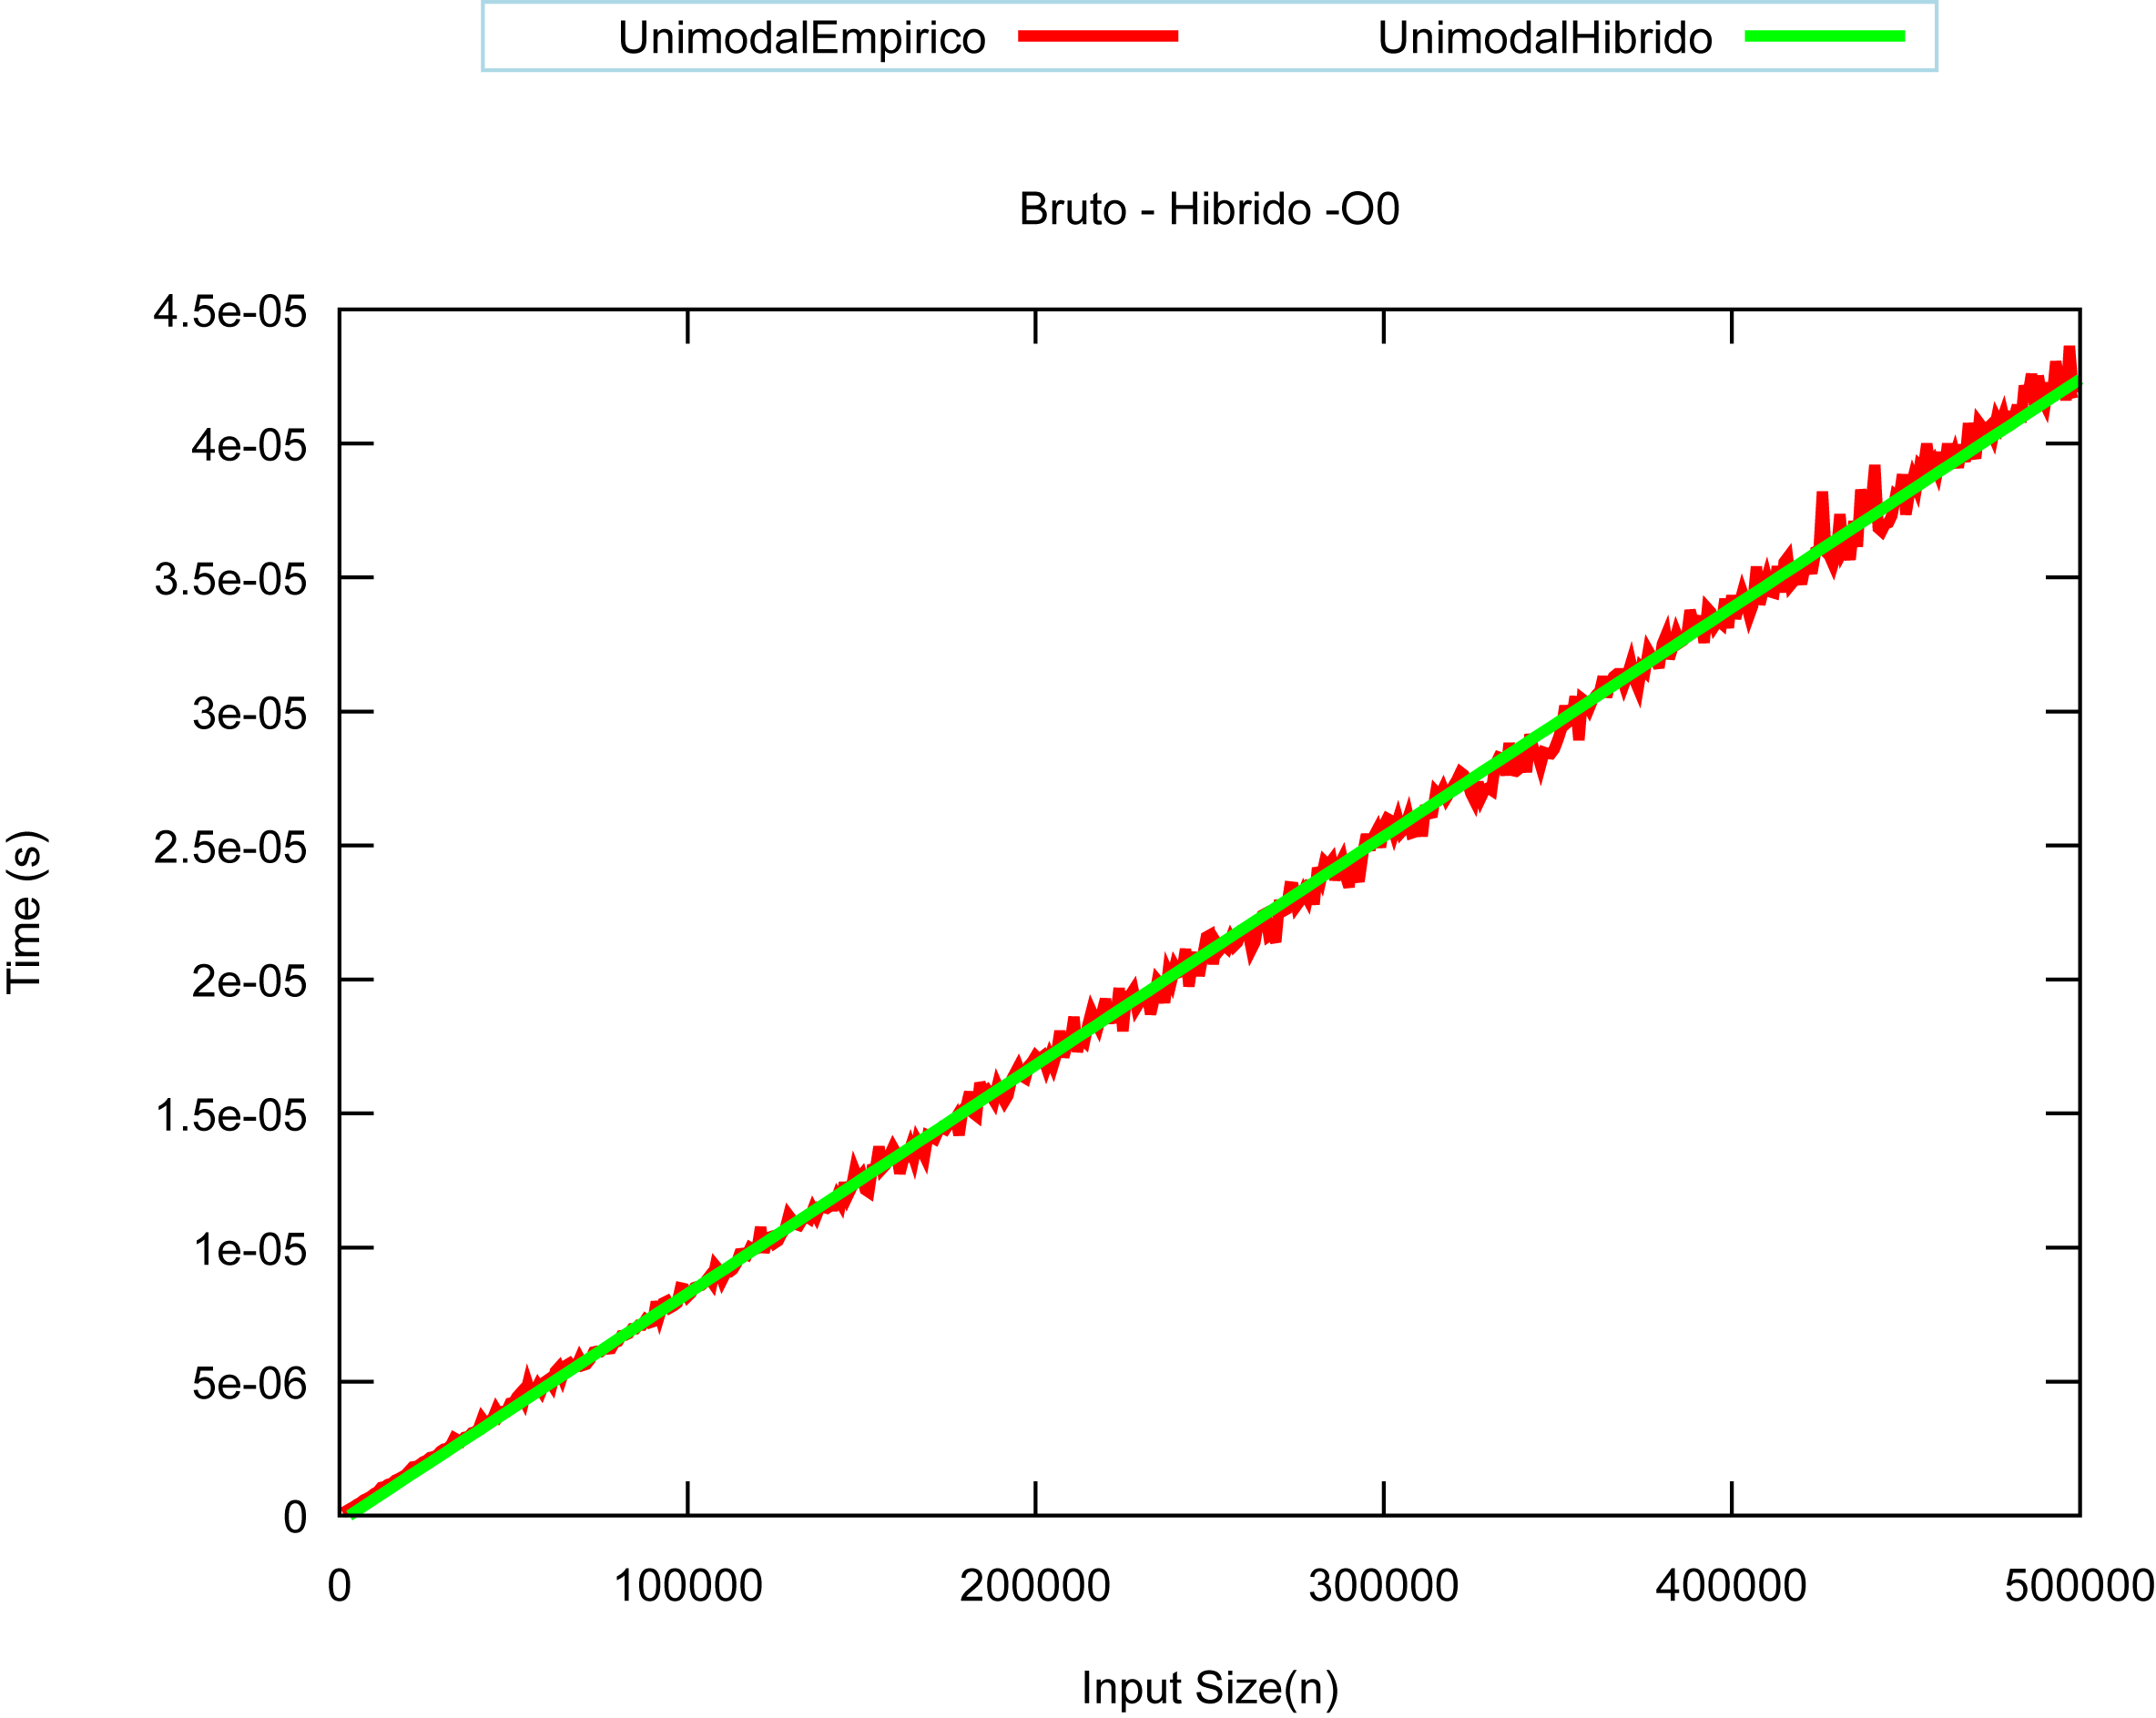
\includegraphics[width=8.6cm,height=7.1cm]{Images/bruto-hibridoO0}}
		\end{picture}
		\end{center}
		\end{figure}
		
\end{frame}	


	
\begin{frame}[plain]
	\frametitle{Constantes ocultas}
	
		\begin{defn}
			
			Sabemos que la función que describe la eficiencia de este algoritmo tiene la siguiente forma:
		\begin{equation}
			T(n)= a\cdot n + b
		\end{equation}
		
		Al realizar el ajuste de los datos con la herramienta \textit{gnuplot} obtenemos el valor de las constantes ocultas, quedando por tanto:
		
		\begin{equation}
			T(n) = 8.5281\cdot 10^{-11} \cdot n -2.43262\cdot 10^{-07}
		\end{equation}
	
		\vspace*{0.05in}
		
	\end{defn}
		
\end{frame}




\begin{frame}[plain]
	\frametitle{Optimización 1}
		\begin{figure}[htb]
		\begin{center}
		\begin{picture}(160,0)
		\put(-50,-110){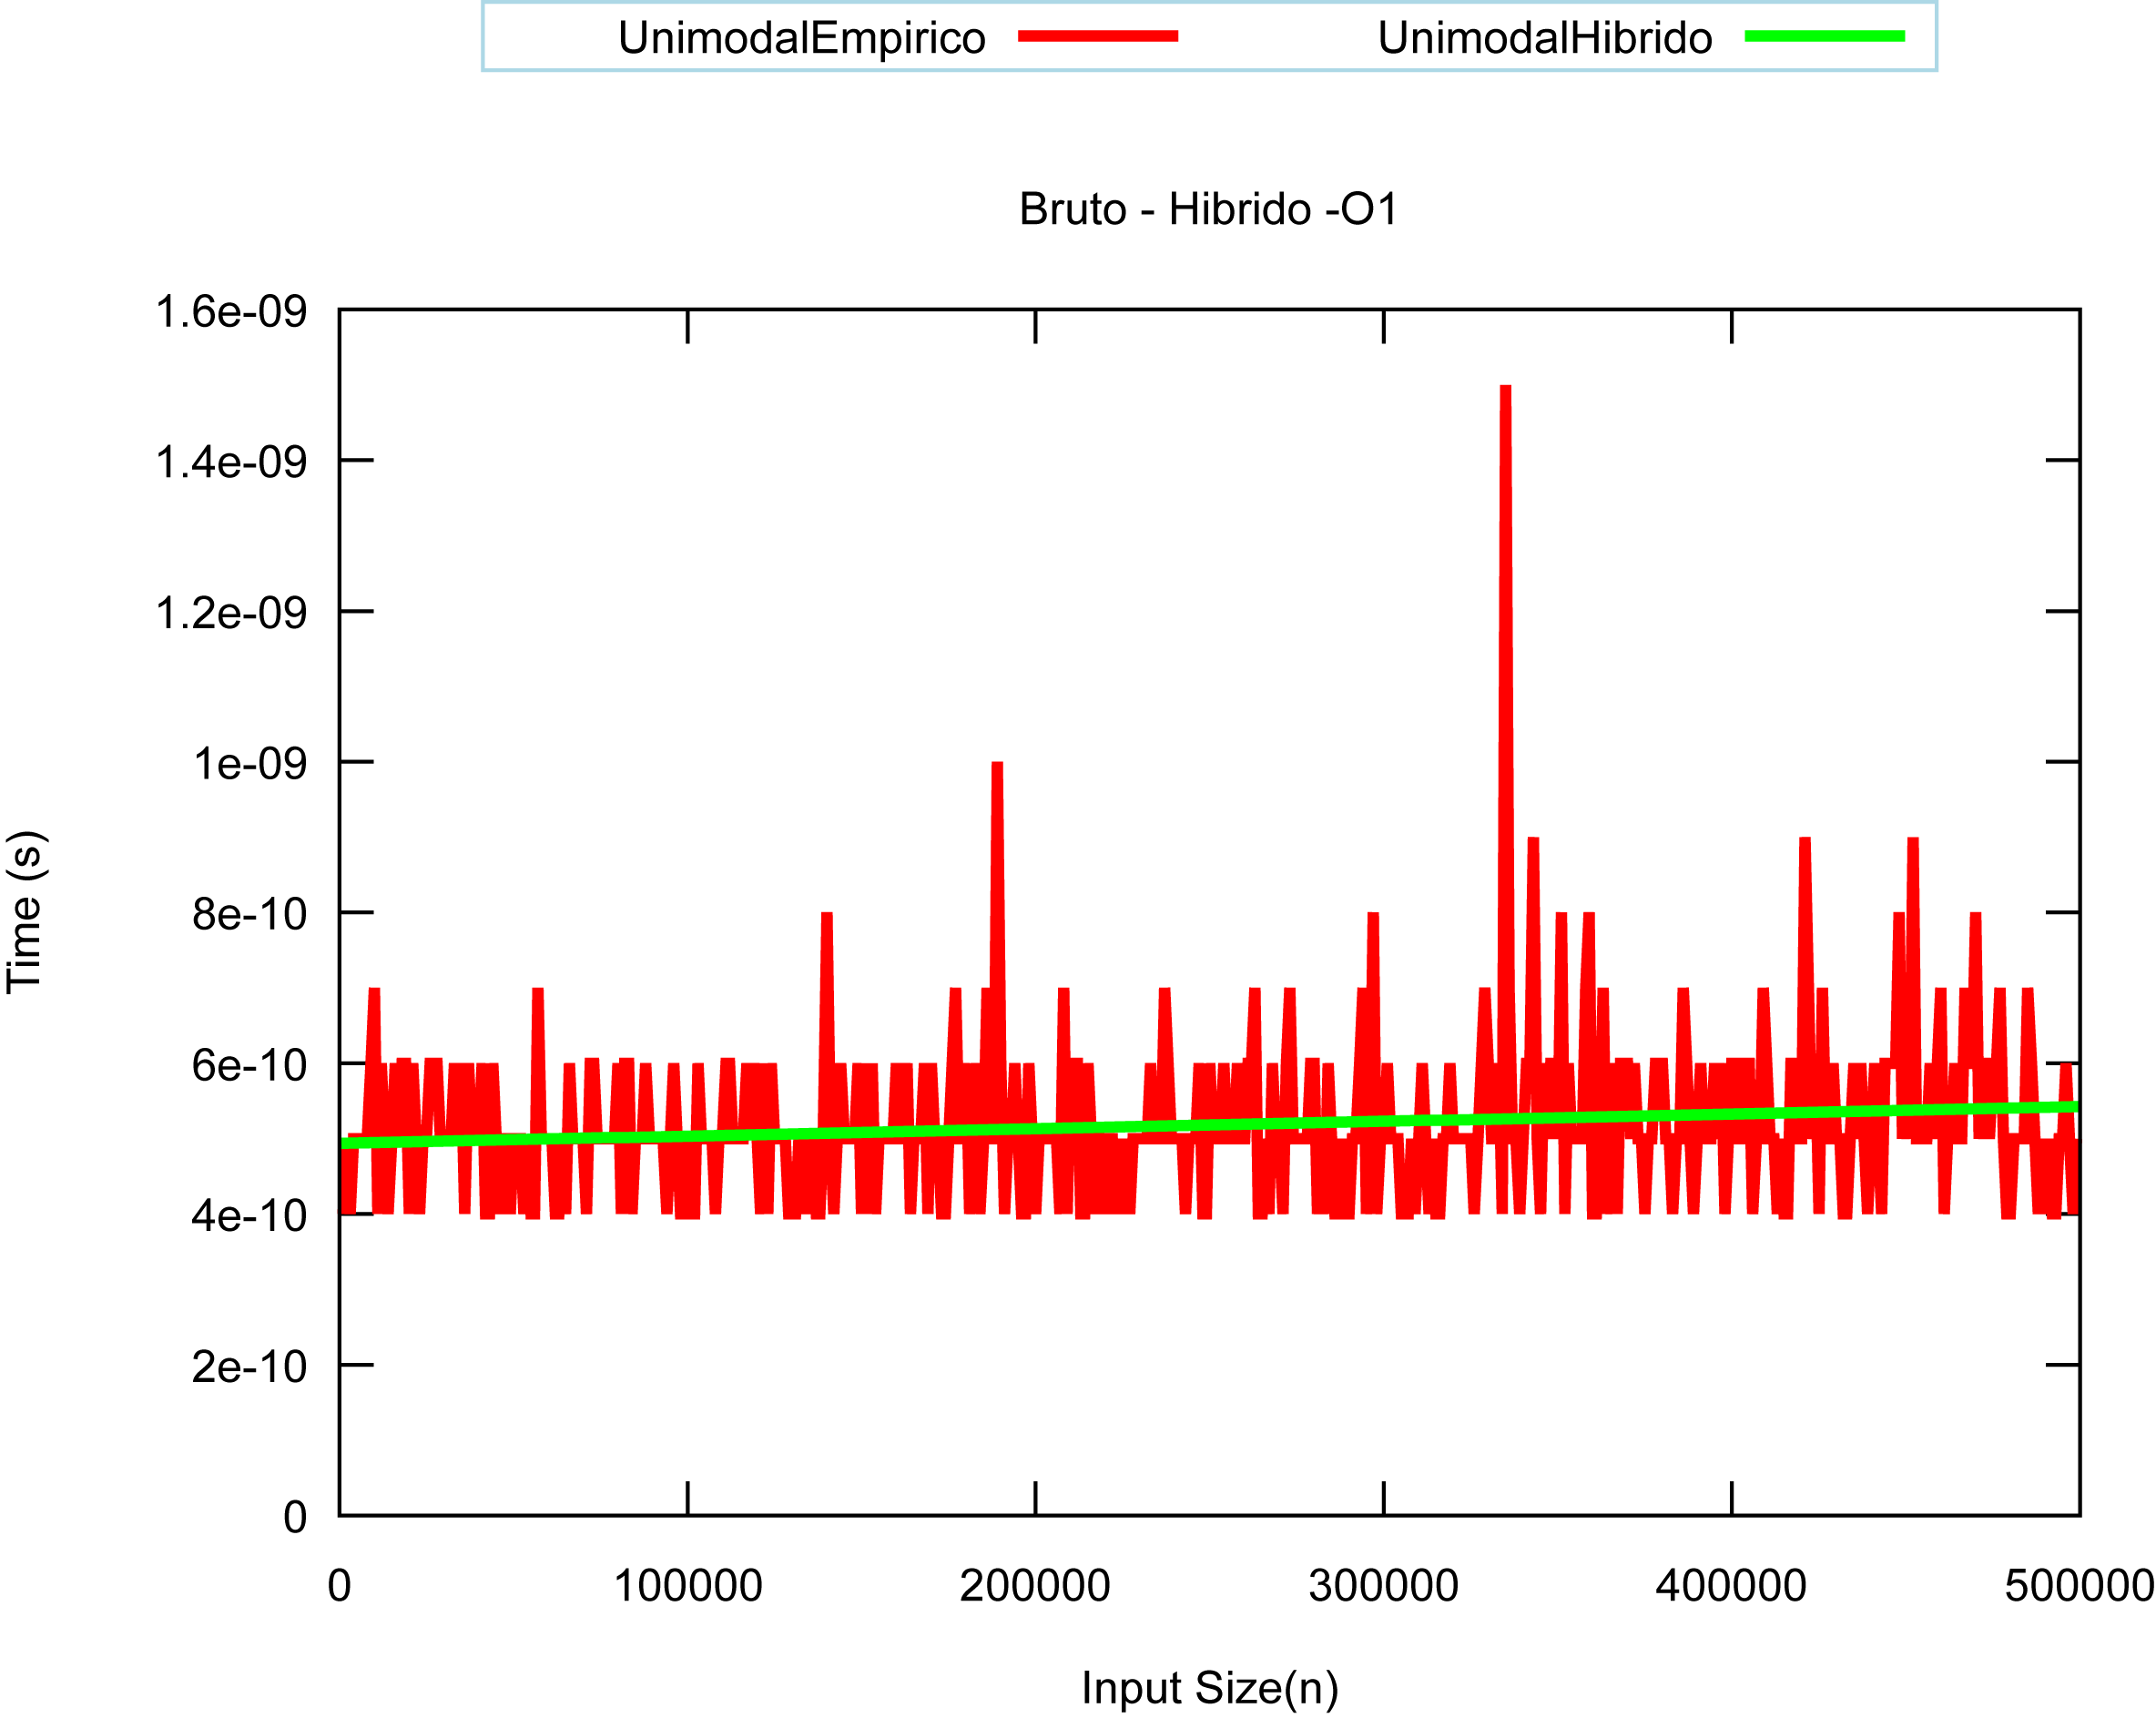
\includegraphics[width=8.6cm,height=7.1cm]{Images/bruto-hibridoO1}}
		\end{picture}
		\end{center}
		\end{figure}
		
\end{frame}	




\begin{frame}[plain]
	\frametitle{Constantes ocultas}
	
		\begin{defn}
			
			En este caso la función queda de la siguiente forma:
		
		\begin{equation}
			T(n) = 9.75348 \cdot 10^{-17} \cdot n + 4.93652 \cdot 10^{-07}
		\end{equation}
	
		\vspace*{0.05in}
		
	\end{defn}
	
	

		
\end{frame}














\begin{frame}[plain]
	\frametitle{Optimización 2}
		\begin{figure}[htb]
		\begin{center}
		\begin{picture}(160,0)
		\put(-50,-110){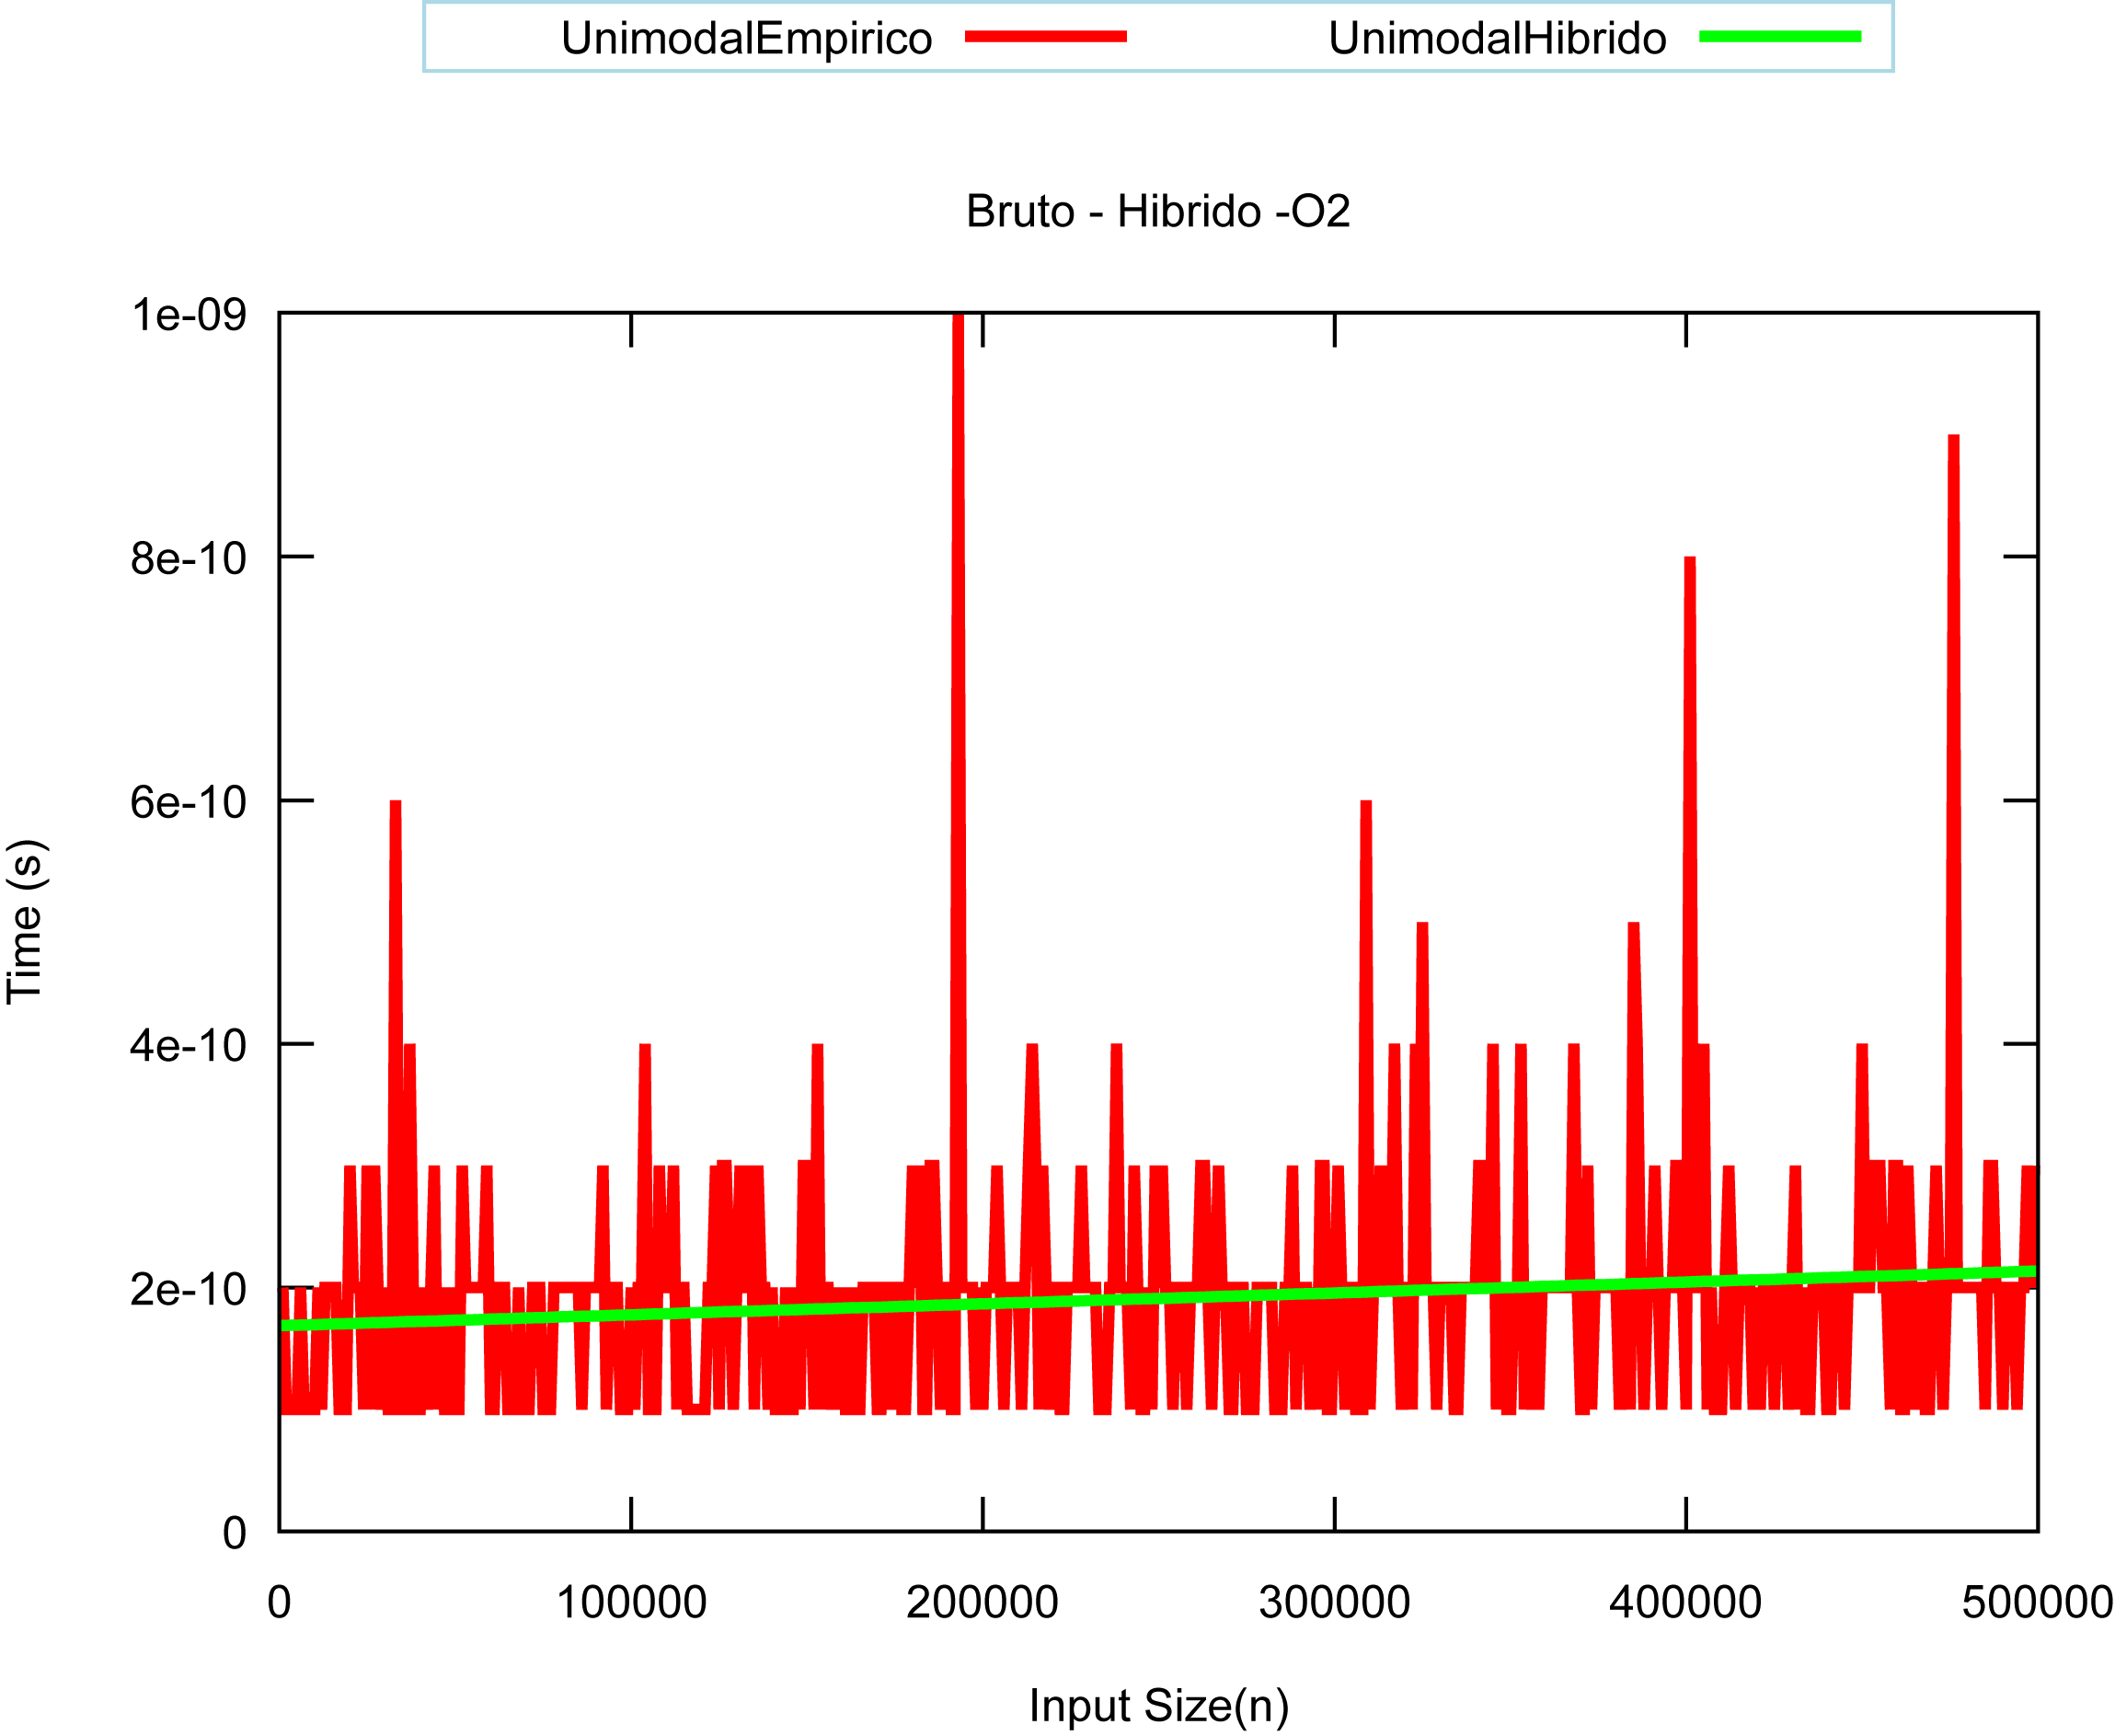
\includegraphics[width=8.6cm,height=7.1cm]{Images/bruto-hibridoO2}}
		\end{picture}
		\end{center}
		\end{figure}
		
\end{frame}	




\begin{frame}[plain]
	\frametitle{Constantes ocultas}
	
		\begin{defn}
			
			En este caso la función queda de la siguiente forma:
		
		\begin{equation}
			T(n) = 8.96154 \cdot 10^{-17} \cdot n + 1.68779 \cdot 10^{-07}
		\end{equation}
	
		\vspace*{0.05in}
		
	\end{defn}
	
	

		
\end{frame}




\begin{frame}[plain]
	\frametitle{Conclusión} 
	
	\begin{exampleblock}{Mejora}
			Como podemos ver, la mejora se encuentra en las constantes ocultas, concretamente, conseguimos una mejora muy sustancial en la pendiente, que pasamos de  $a= 8.5281\cdot 10^{-11}$ a $a =  9.75348e\cdot 10^{-17}$
		\end{exampleblock}
\end{frame}		

		
		
		
		
		
	



